\documentclass{beamer}

\mode<presentation> {
	\usetheme{Darmstadt}
	\usecolortheme{beaver}
}

\usepackage{graphicx}
\usepackage{booktabs}
\usepackage{lmodern}

\setbeamertemplate{blocks}[rounded][shadow=false]
\setbeamerfont{bibliography entry author}{size=\tiny}%
\setbeamerfont{bibliography entry title}{size=\tiny}
\setbeamerfont{bibliography entry journal}{size=\tiny}
\setbeamertemplate{itemize items}[default]
\setbeamertemplate{enumerate items}[default]
\setbeamerfont{bibliography entry note}{size=\tiny}

\newtheorem{proposition}{Proposition}
\newtheorem{hypothesis}{Hypothesis}

\title{Branching Heuristics Promoting Symmetry Activity}

\author{
	J. van Beek \and
	I.J.G. in `t Veen \and
	A.J. Rouvoet \and
	E. Schoute
}
\institute[TU Delft]
{
	Delft, University of Technology \\
	\medskip
	\textit{\{j.vanBeek, a.j.Rouvoet, e.Schoute, i.j.g.intVeen\}@student.tudelft.nl}
}

\date{\today}

\begin{document}

	\begin{frame}
		\titlepage % Print the title page as the first slide
	\end{frame}

	\begin{frame}
		\frametitle{Overview}
		\tableofcontents
	\end{frame}

\section{Background}
	
	\subsection{Research Objective}
	\begin{frame}
		\frametitle{Introduction}
		\begin{block}{Symmetry Propagation}
			A feasible dynamic symmetry breaking technique for SAT-solvers as proposed by
			\cite{devriendt2012symmetry} in 2012.
		\end{block}
	\end{frame}

	\begin{frame}
		\frametitle{Research questions}
		\begin{block}{Hypothesis 1}
			\label{hyp:increased_activity}
			Heuristic $H$ manages to keep more symmetries weakly active during search.
		\end{block}
		
		\visible<+->{
		\begin{block}{Hypothesis 2}
			\label{hyp:activity_equals_speed}
			When more symmetries are active during search, more literals can be propagated, resulting in
			better solve performance on average.
		\end{block}
		}
	\end{frame}

	\subsection{Notation}
	\begin{frame}
		\frametitle{SAT notation}

		\begin{itemize}
			\item Theory $T$ is a conjunction of clauses
			\item Clause $c$ is a disjunction of literals
			\item Literal $l$ is of the form $x$ or $\neg x$ and $x \in \Sigma(T)$
			\item $\Sigma(T)$ is the set of variables in $T$
			\item An assignment $\alpha$ is called a model of $T$ iff it is complete and satisfies
				all clauses of $T$
		\end{itemize}
	\end{frame}

	\subsection{Symmetry}
	\begin{frame}
		\frametitle{Symmetry}

		\begin{definition}[Symmetry]
			Consider a permutation $\sigma$ of a theory $T$. $\sigma$ is called a symmetry if and only if:
			\begin{itemize}
				\item $\sigma(\neg x) = \neg(\sigma(x))$
				\item $\sigma(\alpha)$ is a model for $T$ iff $\alpha$ is a model for $T$
			\end{itemize}
		\end{definition}

		\pause

		\begin{proposition}
			Let $\sigma$ be a symmetry of a theory $T$ and $c$ a clause.
			\begin{equation}
				T \vdash c \quad \implies \quad T \vdash \sigma( c )
			\end{equation}
		\end{proposition}
	\end{frame}

%	\subsection{Symmetry Breaking}
	\begin{frame}
		\frametitle{Symmetry Breaking}

		\begin{itemize}
			\item Static Symmetry Breaking, e.g. Shatter~\cite{aloul2004shatterpb}.
			\item Dynamic Symmetry Breaking, e.g. Symmetry Propagation~\cite{devriendt2012symmetry}.
		\end{itemize}
	\end{frame}

	\subsection{Dynamic Symmetry Breaking}
%	\begin{frame}
%		\frametitle{Dynamic Symmetry Breaking}
%
%		\begin{block}{Approach}
%			Propagate symmetrical literals.
%
%			Given theory $T$, partial assignment $\alpha$ and symmetry
%			\alert<2->{$\sigma$ of $T \cup \alpha$}.
%
%			For each literal $l$:
%			\begin{equation}
%				T \cup \alpha \vdash l \quad
%				\implies
%				\quad T \cup \alpha \vdash \sigma(l)
%			\end{equation}
%
%			Thus when $l$ is progated, $\sigma(l)$ can also be propagated.
%		\end{block}
%	\end{frame}

	\begin{frame}
		\frametitle{Dynamic Symmetry Breaking: Weak Activity}

		\begin{block}<+->{Weak Activity}
			Given a theory T, let $\alpha$ be the current assignment and $\delta$ the set of
			choice literals.
			A symmetry $\sigma$ of T is weakly active if $\sigma(\delta) \subseteq \alpha$
		\end{block}

		\begin{block}<+->{Inactivity}
			Given a theory T, let $\alpha$ be the current assignment and $\delta$ the set of
			choice literals.
			A symmetry $\sigma$ of T is weakly-inactive if $\exists l \in \sigma(\delta), l \not\in \alpha$
		\end{block}
	\end{frame}

\section{Branching Heuristics}

	\subsection{The Idea}
	\begin{frame}
		\frametitle{Symmetry Optimizing Variable Branching}

		\begin{block}{Optimization through literal selection}
			According to Hypothesis 2 improve dynamic symmetry propagation performance by choosing literals that promote
			symmetry weak-activity.
		\end{block}
	\end{frame}

	\subsection{Implemented Heuristics}
	\begin{frame}
		\frametitle{Symmetry Related Variable Branching Heuristics}

		\begin{exampleblock}{Symmetry Activity (SA)}<1->
			\begin{enumerate}
				\item Get first $n$ undecided variables $V$ from the variable heap
				\item For each $v \in V$: perform lookahead on choice literals $v$ and $\neg v$
				\item Continue with branch that has the most weakly-active symmetries
			\end{enumerate}
		\end{exampleblock}

		\begin{block}{Symmetry Activity Approximation (SA-APPROX)}<2->
			Do not do a lookahead.
			Instead assume current choice literals $\delta$, next choice literal $l$, and assignment $\alpha$.
			Let $\alpha' = \alpha \cup \{l\}$ and evaluate the number of active symmetries against that assignment.
		\end{block}

	\end{frame}
	
	\begin{frame}
		\frametitle{Symmetry Related Variable Branching Heuristics}

		\begin{block}{Symmetry Counting}
			Pick $v \in V$ which has the highest amount of symmetries.
		\end{block}

		\visible<+->{
		\begin{block}{Symmetry Usage}
			When a variable is propagated during the Symmetry propagation phase, bump its priority, which may result in the variable moving up in the variable heap.
		\end{block}
		}

	\end{frame}
	
	\subsection{Runtime Analysis}
	\begin{frame}
		\frametitle{Runtime Analysis}
		
		\begin{block}{Symmetry Activity}
			$O(|L|(|T| + |S|))$ per iteration
		\end{block}
		\begin{block}{Symmetry Activity Approximation}
			$O(|S|)$ per iteration
		\end{block}
		\begin{block}{Symmetry Counting}
			$O(|L|)$ preprocessing, hence no effect to overall complexity
		\end{block}
		\begin{block}{Symmetry Usage}
			$O(|S|)$ per symmetry propagation
		\end{block}
	\end{frame}

\section{Results}

	\subsection{Test Procedures}
	\begin{frame}
		\begin{block}{Benchmarks}
			We used the same benchmarks as used by Devriendt et al. for comparison:
			\begin{itemize}
				\item Routing of field-programmable gate arrays: \emph{fpga} and \emph{chnl}.
				\item Pigeonhole problems: \emph{hole}.
				\item Game problems: \emph{battleship}.
				\item Urqhart's problems: \emph{urq}.
			\end{itemize}
		\end{block}
	\end{frame}
	
	\begin{frame}[allowframebreaks]
		\frametitle{Observations}
		\begin{block}{General Observations}
			\begin{itemize}
				\item $SP^{REG}$ and $SP^{OPT}$ perform equally, except on \emph{urq}.
				\item In the \emph{chnl} benchmark, none of the implementations succeed in increasing the number of active symmetries.
				\item The same is the case for \emph{urq}, but that contains only inverting symmetries. %Explain inverting symmetries?
			\end{itemize}
		\end{block}

		\begin{block}{SA Heuristic}
			\begin{itemize}
				\item The SA heuristic was only implemented with a unit propagation lookahead.
					So no symmetry propagation lookahead is performed.
				\item Additionally, it only chooses from the top 5 variables on the heap.
				\item The SA heuristic performs best in keeping the most symmetries active, except in \emph{urq} where $SP^{OPT}$ excels.
			\end{itemize}
		\end{block}

		\begin{block}{Symmetry Counting Heuristic}
			\begin{itemize}
				\item Improved symmetry activity in about $2/3$ of the cases, if we exclude \emph{chnl}.
				\item Performs worse in keeping symmetries active for cases with a lot of inverting symmetries.
			\end{itemize}
		\end{block}

		\begin{block}{Symmetry Usage Heuristic}
			\begin{itemize}
				\item Decreased symmetry activity in most cases, so that Hypothesis 1 is not satisfied.
				\item Probably caused by promoting \emph{all} literals that are part of the used symmetry.
			\end{itemize}
		\end{block}
	\end{frame}
	
	\begin{frame}[plain]
		\frametitle{Active Symmetries During Runtime}
		\begin{figure}
			\centerline{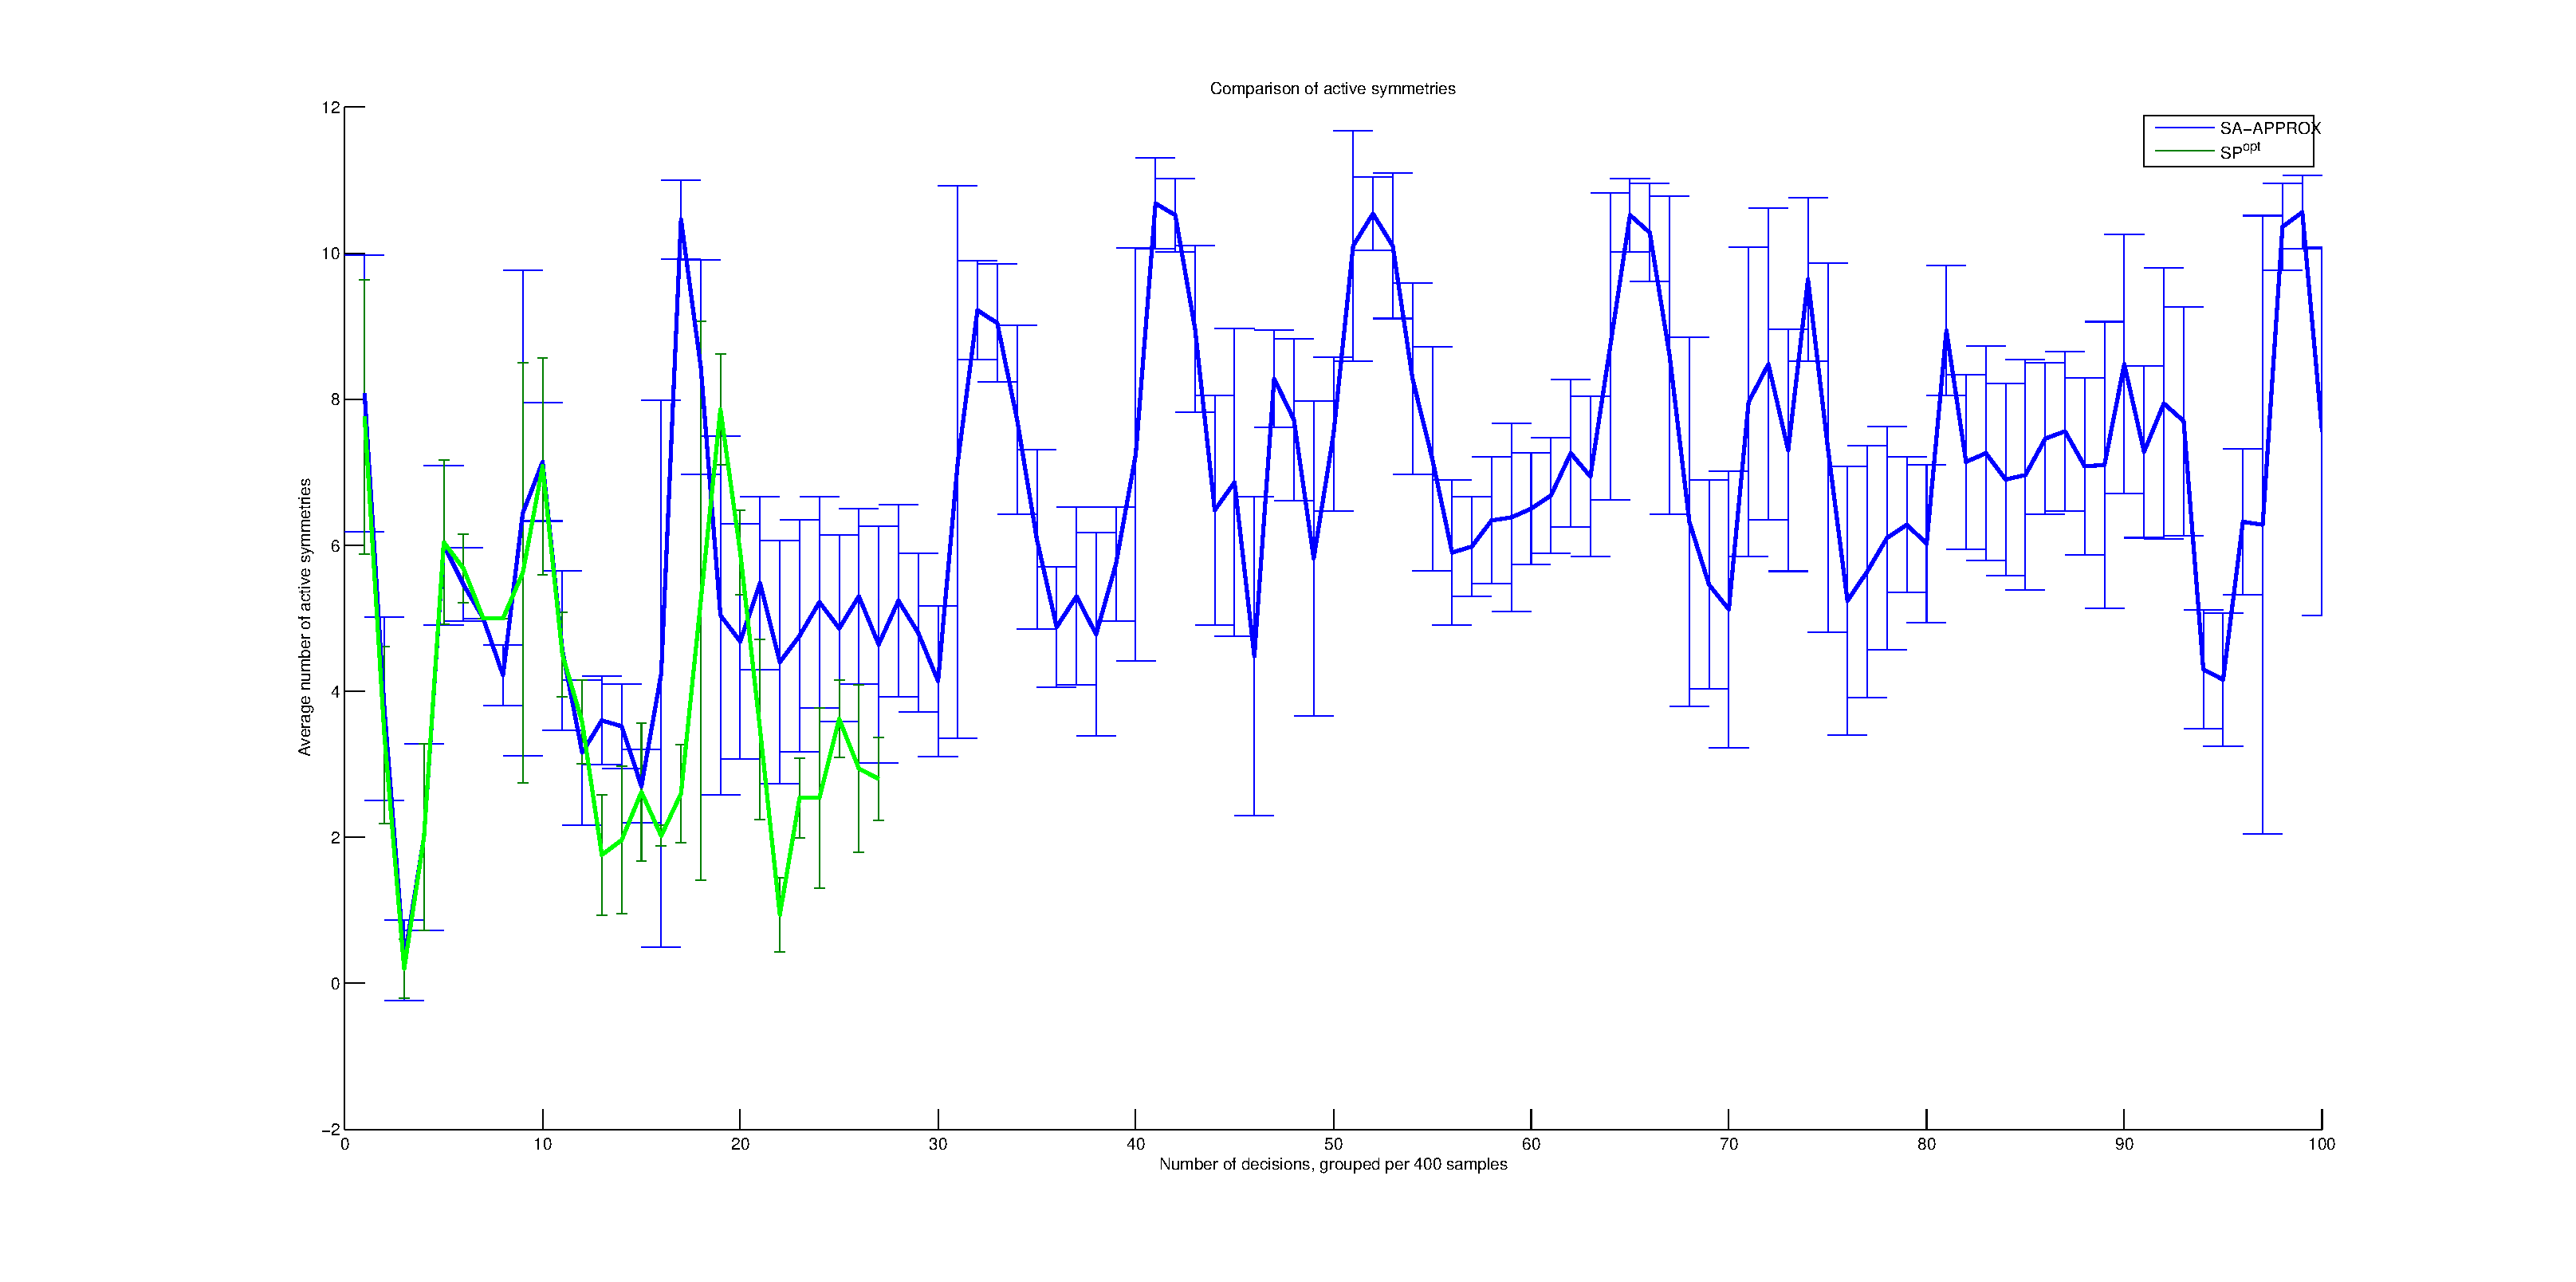
\includegraphics[width=1.2\textwidth]{../results/battleship-12-23-approx-vs-reg.eps}}
			\caption{
				Number of active symmetries during search for one of the cases where SA-APPROX got
				outperformed by $SP^{OPT}$.
				The specific case under test is battleship-12-23
			}
			\label{fig:active_symmetries_during_search}
		\end{figure}
	\end{frame}
	
	\begin{frame}[plain]
		\frametitle{Correlation Performance and Active Symmetries}
		\begin{figure}
			\center
			\centerline{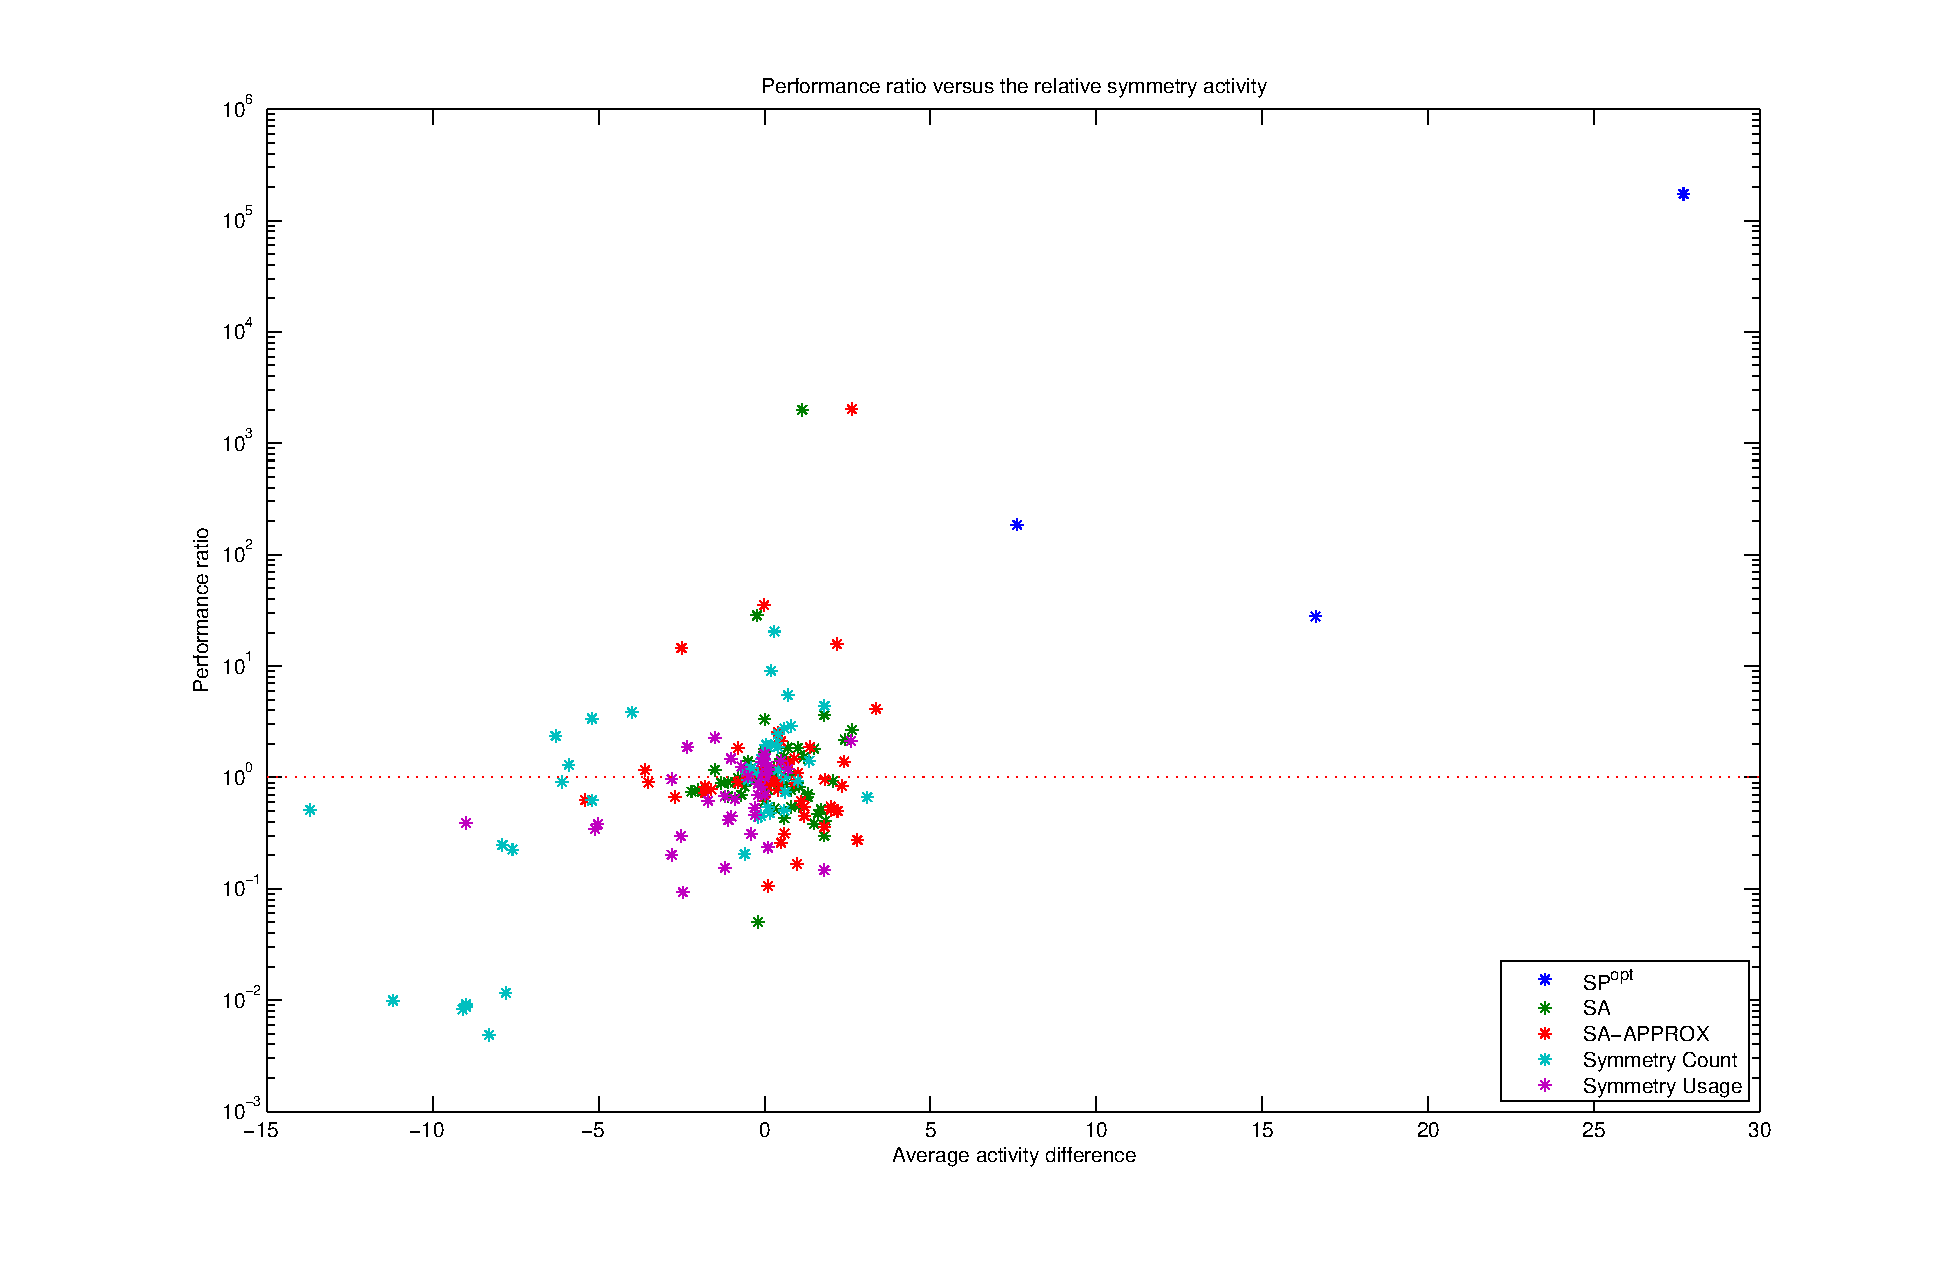
\includegraphics[width=0.9\textwidth]{../results/scatterplot_activity.eps}}
			\caption{
				Correlation between number of active symmetries and number of decisions for all
				heuristics.
				Performance and activity measured relative to $SP^{REG}$.
			}
			\label{fig:correlation}
		\end{figure}
	\end{frame}
	
\section{Conclusion}

	\subsection{Conclusion}
	\begin{frame}
		\frametitle{Conclusion}
		\ldots
	\end{frame}

	\subsection{References}
	\begin{frame}[allowframebreaks]
		\frametitle{References}
		\bibliographystyle{IEEEtran}
		\bibliography{../bibliography}
	\end{frame}

	\begin{frame}
	\Huge{\centerline{Questions?}}
	\end{frame}

\end{document}
